\documentclass[conference]{IEEEtran}
\IEEEoverridecommandlockouts
\usepackage{cite}
\usepackage{amsmath,amssymb,amsfonts}
\usepackage{algorithm}
\usepackage[noend]{algpseudocode}
\usepackage{graphicx}
\usepackage{xcolor}
\usepackage{booktabs}
\usepackage{array}
\usepackage{tikz}
\usetikzlibrary{arrows.meta,positioning,shapes.geometric,fit,calc}
\usepackage[hidelinks]{hyperref}
\usepackage{url}

\newcommand{\msig}{\textsc{Setup\_Signing}}
\newcommand{\prop}[1]{\textsf{#1}}
\newcommand{\code}[1]{\texttt{#1}}
\graphicspath{{../common/figures/}}

\begin{document}

\title{Signed but Unprotected: A Formal and Empirical\\ Study of MAVLink~2 Message-Signing Defaults\\ and Their Bearing on the EU Cyber Resilience Act}

\author{\IEEEauthorblockN{Ian Brighouse}
\IEEEauthorblockA{\textit{Brighouse Security Labs} \\
Spain \\
research@brighousesec.com}}

\maketitle

\begin{abstract}
MAVLink is the de facto command-and-control (C2) protocol of the open-source
drone ecosystem. Since 2016 MAVLink~2 has offered optional per-frame
\emph{message signing}, yet whether a deployed aircraft is actually protected
depends on a tangle of implementation choices---default state, allow-lists,
link exemptions, and a trust-on-first-use key-provisioning step---that, to our
knowledge, no prior work has stated precisely or measured end to end. We make
three contributions.
First, we give a compact parameterised \emph{acceptance semantics} for MAVLink~2
signing: a transition system whose parameters capture the points at which
PX4 and ArduPilot differ, together with a bounded symbolic adversary and six
security properties. Bounded exploration yields short, human-readable attack
witnesses and, crucially, distinguishes an \emph{idealised out-of-band}
provisioning policy---which satisfies every property---from the policies real
stacks implement, which do not. Second, we build three flight stacks from
source (ArduPilot~Copter~4.7.2, PX4~v1.17.0, PX4~v1.18.0-rc1) and audit them in
software-in-the-loop with \emph{mavaudit}, a passive, key-less auditor we
release. We find that \emph{all} default links are unsigned, answer
unauthenticated reads, and expose MAVLink~FTP; that the current \emph{stable}
PX4 release contains no signing implementation at all; and that with signing
enabled ArduPilot's primary channel signs every outbound frame while still
accepting unsigned commands---so a purely passive observer would wrongly judge
it protected. This channel-0 exemption is a documented upstream behaviour
(ArduPilot issue~\#34489, with a fix proposed but not yet merged~\cite{ardupilot_issue34489,ardupilot_pr34780});
our contribution is to measure it independently, to show that the model built
from the implementation reproduces it, and to make explicit that the exemption
follows the channel index rather than the link type (measured by moving the
transport of each channel independently), which motivates an active, read-only
probe. Third, we map each observed property to the essential
requirements of EU Regulation~2024/2847 (the Cyber Resilience Act) and the
command-link requirement of Delegated Regulation~2019/945, producing, to our
knowledge, the first measurable conformance-evidence crosswalk for civil
drones. All code, models, and data are released for reproduction.
\end{abstract}

\begin{IEEEkeywords}
MAVLink, unmanned aerial vehicles, message signing, protocol security, formal
methods, Cyber Resilience Act, secure by default.
\end{IEEEkeywords}

\section{Introduction}
\label{sec:intro}

Open-source flight stacks---principally PX4 and ArduPilot---fly a large and
growing share of commercial and dual-use unmanned aircraft. Both speak
MAVLink, a message protocol designed for constrained radio links whose first
version carried no authentication whatsoever~\cite{marty2014}. Unauthenticated
C2 has been shown repeatedly to enable mission disruption and
takeover~\cite{kwon2018,marty2014}, and the three protocol-level weaknesses are
catalogued as CVE-2020-10281 through CVE-2020-10283. In 2026 a CISA advisory
rated unauthenticated MAVLink in PX4 at CVSS~9.8 (CVE-2026-1579), and a cluster
of memory-safety CVEs in MAVLink file transfer, the MAVLink shell, and log
handlers showed that these sinks are reachable by \emph{any} peer when signing
is off.

MAVLink~2 added optional message signing that addresses integrity and origin
authentication. Ten years later, three questions remain unanswered in the
literature:

\begin{enumerate}
\item \textbf{Semantics.} \emph{When exactly} does a receiver accept a frame?
The specification leaves acceptance of unsigned traffic ``to the
implementation.'' What does that under-specification permit, and which choices
are safe?
\item \textbf{Reality.} How are current releases configured out of the box,
what does enabling signing actually change, and where are the exemptions?
\item \textbf{Consequence.} How do these facts map to the obligations EU drone
manufacturers now carry under the Cyber Resilience Act (CRA) and the UAS
product rules?
\end{enumerate}

\noindent\textbf{Contributions.}
\begin{itemize}
\item A parameterised \emph{acceptance semantics} for MAVLink~2 signing
(Section~\ref{sec:model}), with a bounded symbolic adversary and six properties.
Exploration produces short attack witnesses and shows that an idealised
out-of-band provisioning policy satisfies all six, while the policies PX4 and
ArduPilot implement each violate a distinct subset.
\item An empirical study of three stacks built from source
(Section~\ref{sec:method}--\ref{sec:results}), using \emph{mavaudit}, a
released passive/active auditor. Key findings: insecure by default everywhere;
no signing in stable PX4; and a sign-everything-yet-accept-unsigned behaviour on
ArduPilot's primary channel that only an active probe detects. The behaviour
itself is tracked upstream~\cite{ardupilot_issue34489,ardupilot_pr34780}; what
we add is an independent measurement and a model that reproduces it from the
implementation's own rules.
\item A measurable crosswalk (Section~\ref{sec:cra}) from protocol properties to
CRA Annex~I essential requirements and to the 2019/945 C2-link requirement, i.e.\
conformance evidence a manufacturer can actually produce.
\end{itemize}

All artefacts are available for reproduction.\footnote{Repository and data:
\url{https://github.com/brigghouse/brighouse-autonomy-lab}.}

\section{Background}
\label{sec:background}

\paragraph{Framing} MAVLink~1 frames begin with \code{0xFE} and a six-byte
header; MAVLink~2 frames begin with \code{0xFD}, a ten-byte header, 24-bit
message IDs, and \emph{incompatibility} and \emph{compatibility} flags. The one
defined incompatibility flag, \code{0x01}, marks a signed frame. A per-message
CRC detects mismatched message definitions but is not a security control.

\paragraph{Signing} A signed MAVLink~2 frame carries a 13-byte trailer: an
8-bit link ID, a 48-bit timestamp (units of $10\,\mu$s since 2015-01-01), and a
48-bit truncated SHA-256 over a 32-byte secret key, the header, the payload, the
link ID, and the timestamp. Receivers must reject frames whose per-stream
timestamp does not strictly increase, or that fall more than one minute behind
local time.

\paragraph{What signing does not provide} (i)~\emph{Confidentiality}: payloads
stay in plaintext. (ii)~\emph{Key distribution}: the 32-byte key is pushed with
a \msig{} message \emph{in clear}, to be sent only over a secure link; there is
no rotation, revocation, or per-device identity. (iii)~\emph{Per-sender
identity}: any key holder can sign as any system/component. (iv)~A
\emph{uniform} rule for unsigned traffic: acceptance is implementation-defined.
These four facts are the reason a precise semantics is needed, and they drive
the regulatory analysis in Section~\ref{sec:cra}.

\section{A Parameterised Acceptance Semantics}
\label{sec:model}

We model the receiver $V$ as a transition system over states
$\sigma=(K,\mathit{armed},S,\mathrm{clk})$, where $K$ is the current key (or
$\bot$), $\mathit{armed}$ is the arming flag, $S$ maps each stream
$s=(\mathit{sys},\mathit{comp},\mathit{link})$ to its last accepted timestamp,
and $\mathrm{clk}$ is the local signing clock. A frame is
$f=(\ell,\mathit{src},\kappa,b,k,t,\mathit{id})$ with link $\ell$, claimed
source $\mathit{src}$, kind $\kappa\in\{\textsc{cmd},\textsc{read},\textsc{hb},
\textsc{radio},\textsc{setup}\}$, signed bit $b$, signing key $k$, timestamp
$t$, and link id $\mathit{id}$. Signature verification is abstract: $f$
\emph{verifies} iff $b$ and $k=K$ (no forgery; collisions ignored).

An implementation is a \emph{policy} $\pi$---a tuple of the Boolean/parameter
choices the specification leaves open (Table~\ref{tab:policies}): the set
$\mathsf{trusted}$ of links that never require signatures; the set
$\mathsf{allow}$ of kinds accepted unsigned while keyed; whether the receiver is
\emph{open when unkeyed}; whether it accepts the first key unsigned
(\emph{trust-on-first-use}, TOFU); whether an unsigned \msig{} on a trusted link
may replace the key; whether a signed \msig{} may; and whether \msig{} is
refused while armed. The transition function
$\mathrm{step}_\pi(\sigma,f)\to(\mathit{accept},\sigma')$ is given in
Algorithm~\ref{alg:step}; Fig.~\ref{fig:automaton} shows the decision structure.

\begin{algorithm}[t]
\caption{$\mathrm{step}_\pi(\sigma,f)$: acceptance decision}
\label{alg:step}
\small
\begin{algorithmic}[1]
\If{$\kappa(f)=\textsc{setup}$} \Comment{key management}
  \If{$\pi.\mathsf{setupLinks}\neq{*}\wedge \ell(f)\notin\pi.\mathsf{setupLinks}$}
     \State \Return reject
  \EndIf
  \If{$\pi.\mathsf{refuseArmed}\wedge\sigma.\mathit{armed}$} \State \Return reject \EndIf
  \If{$\sigma.K=\bot$}
     \State \Return $\pi.\mathsf{tofu}$ ? accept, $K{\gets}k'$ : reject
     \Comment{TOFU window}
  \EndIf
  \If{$f$ verifies $\wedge\ \mathrm{fresh}(\sigma,f)\wedge\pi.\mathsf{signedRekey}$}
     \State \Return accept, $K{\gets}k'$ \Comment{signed rotation}
  \EndIf
  \If{$\neg b(f)\wedge\ell(f)\in\pi.\mathsf{trusted}\wedge\pi.\mathsf{unsignedRekey}$}
     \State \Return accept, $K{\gets}k'$ \Comment{console recovery}
  \EndIf
  \State \Return reject
\EndIf
\If{$\sigma.K=\bot$} \State \Return $\pi.\mathsf{openUnkeyed}$ ? accept : reject \EndIf
\If{$\ell(f)\in\pi.\mathsf{trusted}$} \State \Return accept \Comment{link exemption}\EndIf
\If{$b(f)$}
  \State \Return ($k=K\wedge\mathrm{fresh}$) ? accept : reject
\EndIf
\State \Return $\kappa(f)\in\pi.\mathsf{allow}$ ? accept : reject
\end{algorithmic}
\end{algorithm}

\begin{figure}[t]
\centering
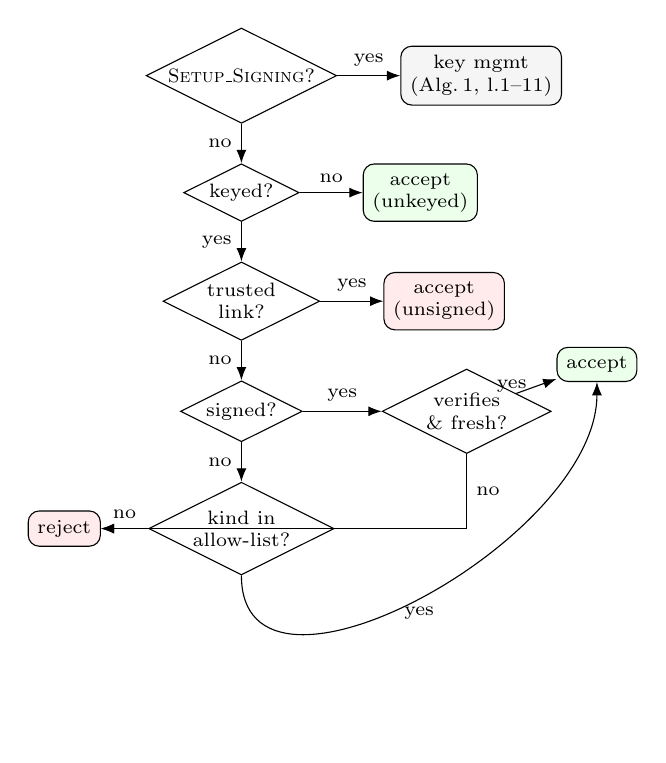
\begin{tikzpicture}[>=Latex,node distance=5mm,
  dec/.style={diamond,draw,aspect=2,inner sep=1pt,font=\scriptsize,align=center},
  act/.style={rounded corners,draw,font=\scriptsize,align=center,fill=black!4},
  lbl/.style={font=\scriptsize}]
\node[dec] (setup) {\msig?};
\node[act,right=8mm of setup] (key) {key mgmt\\(Alg.\,1, l.1--11)};
\node[dec,below=of setup] (keyed) {keyed?};
\node[act,right=8mm of keyed,fill=green!8] (open) {accept\\(unkeyed)};
\node[dec,below=of keyed] (trust) {trusted\\link?};
\node[act,right=8mm of trust,fill=red!8] (texempt) {accept\\(unsigned)};
\node[dec,below=of trust] (signed) {signed?};
\node[dec,right=10mm of signed] (verify) {verifies\\\& fresh?};
\node[act,above right=1mm and 6mm of verify,fill=green!8] (acc) {accept};
\node[dec,below=of signed] (allow) {kind in\\allow-list?};
\node[act,left=6mm of allow,fill=red!8] (rej) {reject};
\draw[->] (setup) -- node[lbl,above]{yes} (key);
\draw[->] (setup) -- node[lbl,left]{no} (keyed);
\draw[->] (keyed) -- node[lbl,above]{no} (open);
\draw[->] (keyed) -- node[lbl,left]{yes} (trust);
\draw[->] (trust) -- node[lbl,above]{yes} (texempt);
\draw[->] (trust) -- node[lbl,left]{no} (signed);
\draw[->] (signed) -- node[lbl,above]{yes} (verify);
\draw[->] (signed) -- node[lbl,left]{no} (allow);
\draw[->] (verify) -- node[lbl,left]{yes} (acc);
\draw[->] (verify.south) |- node[lbl,pos=0.25,right]{no} (rej.east);
\draw[->] (allow) -- node[lbl,above]{no} (rej);
\draw[->] (allow.south) to[out=-90,in=-90] node[lbl,below]{yes} (acc.south);
\end{tikzpicture}
\caption{Decision structure of $\mathrm{step}_\pi$ for an ordinary frame. Red
sinks accept \emph{unsigned} traffic; the link-exemption branch is the one an
active probe is needed to observe (Section~\ref{sec:results}, \prop{R4}).}
\label{fig:automaton}
\end{figure}

\begin{table}[t]
\caption{Policies. Values marked \emph{m} were confirmed against SITL
(Section~\ref{sec:results}); others are documentation-derived and tested by the
conformance run.}
\label{tab:policies}
\centering\footnotesize
\setlength{\tabcolsep}{3pt}
\begin{tabular}{@{}lcccccc@{}}
\toprule
policy & trusted & allow & TOFU & u-rekey & s-rekey & armed \\
\midrule
\textsf{spec-strict}     & $\emptyset$ & \{radio\}   & yes & no  & yes & no  \\
\textsf{ideal-oob}       & $\emptyset$ & \{radio\}   & no  & no  & yes & no  \\
\textsf{px4-1.18}\,(m)   & $\emptyset$ & \{hb,radio\}& yes & no  & yes & yes \\
\textsf{px4-1.17}\,(m)   & all         & ---         & no  & --- & --- & --- \\
\textsf{ardupilot-4.7.2}\,(m) & \{ch0\} & \{radio\}  & yes & yes & yes & no  \\
\bottomrule
\end{tabular}
\end{table}

\subsection{Adversary and properties}
The adversary $A$ sits on one link, can inject any unsigned frame and replay any
frame it has observed on that link, and can sign only with a key it has learned.
Because \msig{} carries the key in clear, $A$ observing provisioning on its link
\emph{learns the key}. $A$ cannot forge. We check six properties by bounded
breadth-first search over $A$'s action sequences, recording the shortest
witness:
\prop{P1} command-integrity (no $A$-command accepted off a trusted link);
\prop{P2} key-integrity ($A$ cannot change $K$);
\prop{P3} replay-resistance;
\prop{P4} first-use window ($A$ installs its own key before provisioning);
\prop{P5} trusted-link exemption ($A$-command accepted on a trusted link);
\prop{P6} key exposure ($A$ on the provisioning link forges afterwards).
\prop{P1}--\prop{P3} are failures; \prop{P4}--\prop{P6} are exposure facts.

\subsection{Results of exploration}
Fig.~\ref{fig:model} summarises the outcome; representative witnesses follow.
\textsf{ideal-oob} is the only policy clean on all six properties and in all
scenarios---closing the TOFU window (no \prop{P4}) removes the key-exposure
chain as well. Every TOFU policy (\textsf{spec-strict}, \textsf{px4-1.18},
\textsf{ardupilot-4.7.2}) exhibits \prop{P4}, and when $A$ sits on the
provisioning link it then achieves \prop{P1}, \prop{P2}, and \prop{P6}: the key
travels in clear, so a three-step trace---observe \msig{}, then sign a command
or a re-key---breaks integrity. \textsf{px4-1.17}, modelled as
\emph{everything-trusted} (no signing code; Section~\ref{sec:results}), shows
\prop{P5} in every post-provisioning scenario and \prop{P3} (no freshness
check). \textsf{ardupilot-4.7.2} additionally shows \prop{P2} with $A$ on the
trusted console link: an \emph{unsigned} \msig{} on \code{ch0} replaces the key.

\begin{figure}[t]
\centering
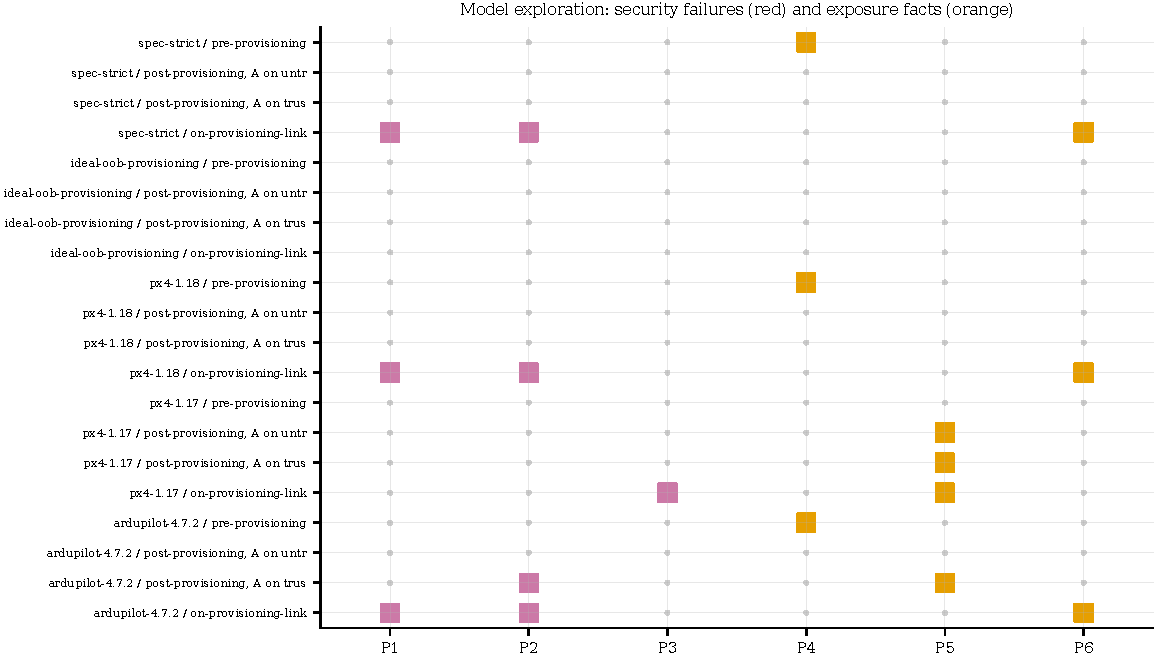
\includegraphics[width=\columnwidth]{fig_model_matrix.pdf}
\caption{Model exploration (depth~3). Red = security failure witnessed; orange =
exposure fact present; dot = not witnessed. \textsf{ideal-oob} is clean
throughout; the implemented policies are not.}
\label{fig:model}
\end{figure}

The take-away for measurement is \prop{R4} below: a policy can sign every
outbound frame yet still accept unsigned input (ArduPilot \code{ch0}). A passive
observer cannot see this; the model tells us precisely which probe does.

\section{Methodology}
\label{sec:method}

\emph{mavaudit} classifies each observed frame from its raw header bytes
(MAVLink~1; unsigned MAVLink~2; signed MAVLink~2 via flag \code{0x01}) and
identifies the autopilot from \textsc{heartbeat}. It never needs the key. With
an \emph{active probe} it sends two unsigned, read-only requests to the first
autopilot seen: a \textsc{param\_request\_read} for parameter index~0
(name-independent across releases---ArduPilot~4.7 renamed \code{SYSID\_THISMAV}
to \code{MAV\_SYSID}) and a \textsc{command\_long} requesting
\textsc{autopilot\_version} (firmware and capability flags). Only replies for
index~0 from the probed vehicle count; the \textsc{command\_ack} is recorded as
corroboration. A scope guard restricts targets to loopback/private addresses and
checks the sending peer before probing; an active probe on a serial port
(which could egress over a radio) requires explicit authorisation. The tool is
validated against a reference vehicle in unsigned, signed, signing-exempt, and
MAVLink~1 modes.

We built three stacks from source on one headless Ubuntu~24.04 VM:
ArduPilot~Copter~4.7.2 (\code{fb77356789}), PX4~v1.17.0 (\code{d6f12ad1c4}, the
latest stable), and PX4~v1.18.0-rc1 (\code{fca3df865a}). PX4 runs with its
built-in SIH physics; no hardware, no RF. For each link we (i)~audit the default
configuration, (ii)~provision the lab key as an operator would (an unsigned
\msig{} over the local link), (iii)~audit again, and (iv)~verify signatures with
the key. For PX4 we also test that an unsigned re-key is rejected.

\section{Measurement Results}
\label{sec:results}

Fig.~\ref{fig:default} and Table~\ref{tab:results} give the measured data.

\begin{figure}[t]
\centering
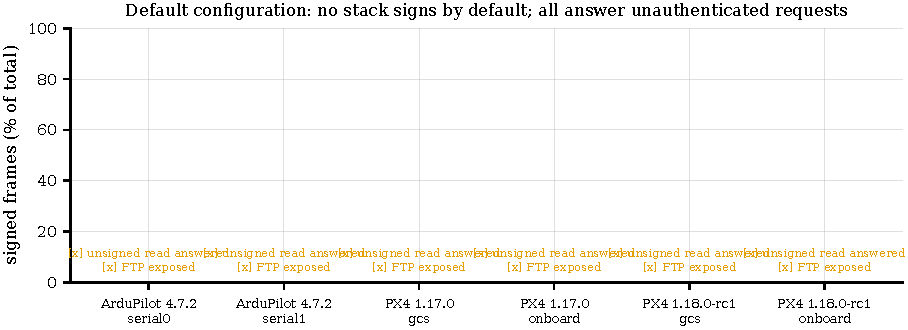
\includegraphics[width=\columnwidth]{fig_default_posture.pdf}
\caption{Default configuration of all three stacks: zero signed frames; every
link answers the unauthenticated read and exposes MAVLink~FTP.}
\label{fig:default}
\end{figure}

\begin{figure}[t]
\centering
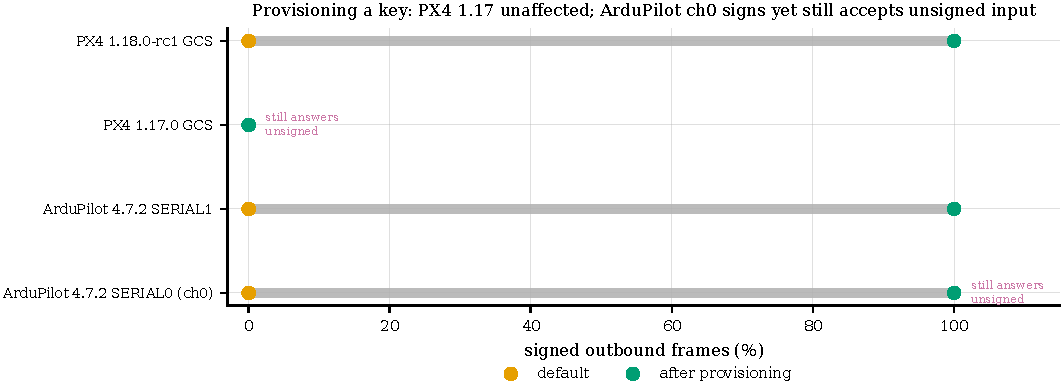
\includegraphics[width=\columnwidth]{fig_provisioning.pdf}
\caption{Before vs after provisioning. PX4~1.17 is unchanged (no signing code).
ArduPilot \code{ch0} and both PX4~1.18 links reach 100\% signed, but \code{ch0}
and PX4 differ on whether unsigned input is still accepted.}
\label{fig:prov}
\end{figure}

\begin{table}[t]
\caption{Measured outcomes. ``u-read'' = unsigned read answered; ``keyed'' =
signatures verified / frames decoded.}
\label{tab:results}
\centering\footnotesize
\setlength{\tabcolsep}{3.5pt}
\begin{tabular}{@{}llcccc@{}}
\toprule
stack & link & \multicolumn{2}{c}{default} & \multicolumn{2}{c}{provisioned}\\
      &      & signed & u-read & signed & u-read \\
\midrule
ArduPilot 4.7.2 & SERIAL0 (ch0) & 0\% & yes & 100\% & \textbf{yes} \\
ArduPilot 4.7.2 & SERIAL1       & 0\% & yes & 100\% & no \\
PX4 1.17.0      & GCS           & 0\% & yes & 0\%   & yes \\
PX4 1.17.0      & Onboard       & 0\% & yes & 0\%   & yes \\
PX4 1.18.0-rc1  & GCS           & 0\% & yes & 100\% & no \\
PX4 1.18.0-rc1  & Onboard       & 0\% & yes & 100\% & no \\
\bottomrule
\end{tabular}
\end{table}

\paragraph{\prop{R1}: insecure by default, everywhere} On all six default links:
zero signed frames, the unauthenticated read answered, and MAVLink~FTP
advertised. A stack shipped unchanged provides a C2 link with neither integrity
nor access control.

\paragraph{\prop{R2}: stable PX4 cannot sign} In v1.17.0 the provisioning step
had no effect---no key file, zero valid signatures, reads still answered. Source
inspection agrees: the v1.17.0 MAVLink module contains no signing implementation
and no \code{MAV\_SIGN\_CFG} parameter. The CISA remediation for CVE-2026-1579
(``enable signing'') is thus unavailable on stable PX4; it first appears in the
v1.18 line. This corrects a claim in our own earlier survey and, we believe, a
plausible misreading of the v1.18 release notes.

\paragraph{\prop{R3}: PX4 v1.18 signing matches its documentation} After
unsigned first-use provisioning: a 40-byte key file appears; 100\% of outbound
frames are signed on both links and every decodable frame verifies; the unsigned
read and version request go unanswered; and a later \emph{unsigned} attempt to
install a different key is rejected while the original key stays valid. The TOFU
window before the first key remains (model \prop{P4}).

\paragraph{\prop{R4}: ArduPilot's channel-0 exemption hides from passive
observers} With a key installed, SERIAL1 signs everything and ignores unsigned
input. SERIAL0 also signs every outbound frame (Fig.~\ref{fig:passive}), yet
still answers the unsigned read and acknowledges the unsigned command request.
This is by design: \code{accept\_unsigned\_callback} returns true on
\code{MAVLINK\_COMM\_0}, ``assumed to be secure channel \ldots USB on ChibiOS
boards.'' An auditor watching only traffic would conclude the link is protected.
The model named this case (\prop{P5}; Fig.~\ref{fig:automaton}, red
link-exemption sink), which is why mavaudit's finding relies on an active
read-only probe and states the discrepancy explicitly. A model-based conformance
run~\cite{brighouse2026formal} confirms it: over eight read-only probe cases the
stack's behaviour matches the model exactly ($8/8$), including the keyed
trusted-link case in which an unsigned read is answered.

\emph{Index, not transport.} Because the exemption is justified by the
assumption that channel~0 is USB, we checked whether it follows the channel
index or the link type by moving the transport of each channel independently
(Table~\ref{tab:ch0}). With SERIAL0 carried over UDP instead of TCP the keyed
channel still answers unsigned reads; with SERIAL1 carried over the same UDP
transport it rejects them. The two runs differ only in which channel index the
UDP link occupies, so the exemption is a property of the index. On any board
whose SERIAL0 is a telemetry radio or a network port rather than USB, that port
accepts unsigned commands while every other port is protected---the situation
described in the upstream issue~\cite{ardupilot_issue34489}, now measured. A
fourth configuration sets \code{SERIAL1\_PROTOCOL}=1 (MAVLink~1): the
documentation states such ports are ``not protected,'' but in 4.7.2 a keyed
MAVLink~1 port rejects an unsigned MAVLink~1 read (the frame cannot carry a
signature and the channel is not channel~0); we report the measurement, which is
stricter than the text. All 23 observations agree with the policy.

\begin{table}[t]
\caption{Channel-0 exemption vs.\ transport, ArduPilot 4.7.2 SITL, key active,
unsigned \code{PARAM\_REQUEST\_READ}. Recorded in \code{results/ch0-configs}.}
\label{tab:ch0}
\centering
\begin{tabular}{llll}
\toprule
Config & SERIAL0 (ch0) & SERIAL1 (ch1) & unsigned read answered \\
\midrule
A & TCP & TCP & ch0 yes, ch1 no \\
B & \textbf{UDP} & TCP & ch0 \textbf{yes}, ch1 no \\
C & TCP & \textbf{UDP} & ch0 yes, ch1 \textbf{no} \\
D & TCP & TCP, MAVLink~1 & ch0 yes, ch1 no (MAVLink~1 probe) \\
\bottomrule
\end{tabular}
\end{table}

\begin{figure}[t]
\centering
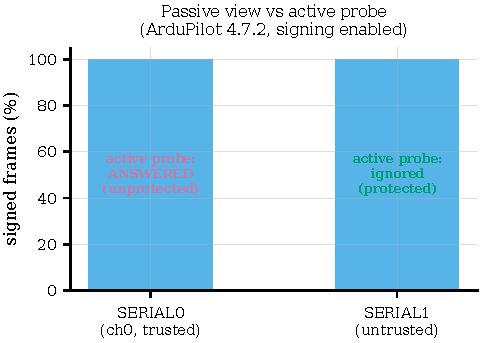
\includegraphics[width=0.78\columnwidth]{fig_passive_vs_active.pdf}
\caption{ArduPilot 4.7.2 with signing enabled. Both links sign 100\% of outbound
frames (passive view identical); only the active probe reveals that \code{ch0}
still accepts unsigned input.}
\label{fig:passive}
\end{figure}

\paragraph*{A second control plane the key does not cover}
Signing protects MAVLink links, and a deployment that has provisioned a key may
reasonably believe its command path is authenticated. PX4 ships a second one.
The \code{uxrce\_dds\_client} module is included in SITL and most firmware
builds and started by the stock init script; it bridges uORB to a DDS network,
and PX4's documentation states that the transport is unauthenticated and reaches
uORB directly. We measured the consequence passively: binding the configured
agent port and decoding what arrives, without answering. Both PX4~v1.17.0 and
v1.18.0-rc1 emit repeated XRCE \code{GET\_INFO} submessages addressed to
\code{OBJECTID\_AGENT} in a session with no client key---agent discovery offered
to whichever process holds the port, with no credential, key or challenge
preceding it, and no means for the client to authenticate the agent that
answers. We did not answer, so no session was established and no topic was read
or written; this is detection, not exploitation, and we claim nothing about what
a full agent could then do beyond what PX4 documents. The same probe against
ArduPilot~4.7.2 returns nothing and the build exposes no \code{DDS\_ENABLE}
parameter, so its DDS subsystem is not compiled in---a property of that build,
since the source defaults the parameter to enabled where it is compiled.

The point for conformance is not that this is a defect; it is documented. The
point is that \emph{the key does not reach it}. A technical file that records
``message signing enabled'' as evidence for Annex~I~2(d) is incomplete if a
second, unauthenticated path to the same vehicle state ships in the same binary.

\section{From Protocol Properties to CRA Evidence}
\label{sec:cra}

The CRA (Regulation~(EU)~2024/2847) applies to products with digital elements
that have a data connection; it excludes products \emph{certified} under
aviation Regulation~2018/1139, but open-category drones carrying a C-class mark
under Delegated Regulation~2019/945 undergo conformity assessment, not
certification, and are thus in scope, as is commercially distributed GCS
software. A manufacturer integrating PX4 or ArduPilot carries the full Annex~I
obligations for the whole product. This is a technical interpretation, not legal
advice. Table~\ref{tab:cra} maps each measured observation to the Annex~I
essential requirement it bears on, to the 2019/945 C2-link requirement, and to
the concrete evidence a manufacturer can produce with the released tooling.

\begin{table}[t]
\caption{Crosswalk: protocol observation $\to$ CRA Annex~I, Part~I(2) $\to$
evidence. A \emph{mavaudit} report ($\downarrow$ severity) is machine-checkable
conformance evidence.}
\label{tab:cra}
\centering\footnotesize
\setlength{\tabcolsep}{3pt}
\renewcommand{\arraystretch}{1.15}
\begin{tabular}{@{}p{2.5cm}p{2.3cm}p{2.5cm}@{}}
\toprule
observation & Annex~I, Part~I(2) & evidence \\
\midrule
no signed frames & (b) secure by default; (d) access; (f) integrity &
100\% signed; provisioning procedure \\
answers unsigned read & (d); (j) attack surface &
MAV-005 absent (active probe) \\
MAVLink~1 on radio port & (b); (f) &
no v1 frames observed \\
no confidentiality & (e) confidentiality &
encrypted datalink, risk-justified \\
FTP/shell exposed & (a) no known exploitable vuln.; (j) &
services gated; SBOM + CVE watch \\
unsigned firmware & (f) integrity of programs &
secure-boot configuration \\
no vuln.\ handling & Part~II(5)--(6); Art.~14 &
CVD policy; ENISA runbook \\
\bottomrule
\end{tabular}
\end{table}

The crosswalk is operational: each row is a finding mavaudit emits with a
severity, so a CI gate (\code{mavaudit scan \texttt{-{}-}fail-on high}) turns the
CRA's ``secure by default'' requirement into a build-time check. The 2019/945
Part~3 requirement that a class-C2/C3 command link be ``protected against
unauthorised access'' is outcome-only; our measurements show that MAVLink
signing is a candidate mechanism but that, under \prop{R4}, signing alone can
fail a strict reading. The forthcoming EU Trusted Drone label and Drone Security
Package~\cite{ec2026droneactionplan} may specify the C2-link property more
concretely; a measurable crosswalk such as ours is a candidate evidence basis.

\section{Discussion and Limitations}
\label{sec:discussion}

The study is simulation-only; vendor firmware and hardware radios may differ.
Our legal reading tracks public texts as of November~2026. We report four
defensive recommendations in priority order: (i)~ship with signing enabled or an
unavoidable first-run provisioning step, closing the TOFU window and preferring
out-of-band keys (model: move from \textsf{spec-strict} toward \textsf{ideal-oob});
(ii)~choose a stack version that can sign and treat any trusted/console link as
unauthenticated; (iii)~add link confidentiality where the risk assessment
requires it; (iv)~audit \emph{actively}, since a link that signs everything may
still accept unsigned input (\prop{R4}).

\section{Related Work}
\label{sec:related}

Foundational MAVLink security analyses~\cite{marty2014,kwon2018} and the MAVSec
encryption proposal~\cite{allouch2019} established the threat but predate the
signing deployment we measure. Fuzzing of flight
stacks~\cite{kim2019rvfuzzer,kim2021pgfuzz} shows that authentication is
necessary but not sufficient. Surveys~\cite{hamza2024,nassi2021} catalogue
threats without a formal acceptance model or longitudinal measurement. Published
regulatory crosswalks operate at the process level---CRA to
ATT\&CK and to GDPR~\cite{ruohonen2025sok,ruohonen2025gdpr}, UNECE~R155 to
ISO/SAE~21434~\cite{costantino2022r155}, DO-326A to avionics
architecture~\cite{siddiqui2023do326a}---and none maps essential requirements to
\emph{measurable protocol properties} of a drone C2 link or produces evidence by
executing checks against the implementation. MAVLink~2 itself has been verified
formally before: PAVE-MAVLink analyses it in ProVerif and validates the result
empirically, over the air, on a physical PX4
aircraft~\cite{wray2025pave,wray2025pavedemo}, proposing an added ChaCha20 layer
as the remedy. We claim neither priority in verifying the protocol nor in testing
against real hardware. What we have not found in prior work is a semantics
\emph{parameterised} by the points on which implementations differ---so that the
stacks become instances to compare rather than separate case studies---or a
conformance crosswalk that produces CRA evidence by executing checks against the
implementation. We say this from published abstracts and metadata, the MILCOM
proceedings being paywalled, and will revise it if the full texts show
otherwise.

\section{Conclusion}
\label{sec:conclusion}

MAVLink signing works when enabled: PX4~v1.18.0-rc1 and ArduPilot~4.7.2 SERIAL1
enforce it as documented. But it is off by default in every stack we tested,
absent from the current stable PX4 release, and bypassed by design on
ArduPilot's primary channel in a way no passive observer can see---a case our
formal model predicts. For EU manufacturers the CRA turns this integrator
responsibility into a legal obligation with live reporting duties. A reproducible
audit that pairs passive observation with a read-only active probe is a cheap,
machine-checkable first piece of conformance evidence.

\section*{Availability and Ethics}
All code, models, and data are released under permissive licences for
reproduction. The work is defensive: no exploit code, attack automation, or RF
tooling is included, and only self-hosted simulators were tested. The
channel-0 signing exemption discussed here was already public upstream before
this work (issue~\#34489 and the unmerged fix in PR~\#34780~\cite{ardupilot_issue34489,ardupilot_pr34780});
we therefore claim no new vulnerability, and no embargo applies. Our
measurements are public and may be cited in that discussion.

\bibliographystyle{IEEEtran}
\bibliography{../common/refs}

\end{document}
